\section{Literature Review}

\subsection{Motor-sport Aerodynamics}
In 1949 Ludwig Prandtl stated: "the term aerodynamics is generally used for the problem arising from flight and other topics involving the flow of air" \cite{Anderson2010FundamentalsAerodynamics}. By this definition, aerodynamics is one of the branches in physics which concerns and studies the interaction of a body and a fluid flow \cite{Scibor-Rylski1984RoadAerodynamics}. The magnitude and direction of the forces that occur on a body result from flow interactions which depend on several geometric variables. Some fundamental variables in aerodynamics include flow velocity, temperature, pressure, and density. Drag and lift are the most significant considerations in race-car aerodynamics, and these will be discussed further in the following sections.

\noindent Aerodynamics is generally divided into external (flow around the body) and internal (flow inside the body). This report will concentrate on external aerodynamics, which focuses on the generation of force due to the airflow around the body of interest. In the automotive industry, external forces play an integral role, since the car's overall performance depends greatly on the aerodynamic forces. These significantly influence the design of the vehicle shape to help maximise aerodynamic advantage \cite{Scibor-Rylski1984RoadAerodynamics}. Some aerodynamic considerations for a vehicle's shape include: large downforce generation; force balance between front and rear tyres; and drag minimisation. Table~\ref{Table1} shows the effect of downforce on a racing car's acceleration: it can be seen that developing downforce significantly improves the acceleration time by -1.06 seconds, the rate of acceleration by 4.5 $m/s^2$, and the power transferred by 124 kilowatts. 

\begin{table}[!ht]
\caption{\label{Table1} Aerodynamics Downforce Effect On a Racing Car's Performance \cite{Scibor-Rylski1984RoadAerodynamics}.}
\vspace{-5mm}
\begin{center}
 \begin{tabular}{||c| c| c ||} 
 \hline
 Variables & With Downforce & Without Downforce \\ [0.5ex] 
 \hline\hline
 Time from 0 to 160 $km/h$ & 5s & 6.06s \\ 
 \hline
 Rate of acceleration at 44 $m/s$ & 10.02 $m/s^{2}$ & 5.52 $m/s^2$ \\
 \hline
 Power transferred at 44 $m/s$ & 353 kW & 229 kW  \\
 \hline
\end{tabular}
\end{center}
\end{table}

\noindent Queen's Formula Racing has been focusing on aerodynamics since 2016. Previous students have attempted to analyse earlier iterations of the QFR car, including the undertray, to optimise the overall performance. This report focuses solely on external aerodynamics in order to understand the QFR undertray's flow behaviour and the mechanisms through which it generates forces. These analyses are then used to inform geometrical consideration of the final aerodynamic undertray design.

\subsection{Aerodynamics Fundamentals}
To fully understand the flow physics and behaviour of the aerodynamic undertray, there are several fundamental aspects and some aerodynamic terminology which first need to be understood.

\subsubsection{Flow Types}
The main characteristic of a gas is the ability of the molecules to move around space freely. The gas molecule's movement to another point in space also requires energy, mass, and momentum to be transferred with it. During this process, a "transfer phenomena" has occurred, where the molecule's movement has introduced viscosity (friction), thermal conduction, and mass diffusion \cite{Anderson2010FundamentalsAerodynamics}. Flows that show evidence of these "transfer phenomena" can be called viscous flows. On the other hand, flows in which these "transfer phenomena" do not occur are known as inviscid flows.

\noindent Some flows, such as those of streamlines far from walls, can be represented as inviscid. But to capture the aerodynamic behaviour that takes place between two walls, such as seen in an undertray, viscosity plays a crucial role. The shear stress near wall boundaries occurs due to this viscosity, which represents one of the significant sources of drag. The presence of viscosity also causes flow separation to take place on high incidence geometries. The viscous effect is therefore an essential consideration in the analysis where the body of interest is purposely designed to generate aerodynamic forces due to the flow, such as in airfoils and undertrays.

\noindent Another vital property in aerodynamics is the density ($\rho$). The compressibility of a flow refers to changes induced in the density by the flow field. Incompressible flow refers to flows with constant density throughout, which is usually seen at Mach numbers less than 0.3. In contrast, flows with regions in which the Mach number is greater than 0.3 are known as compressible flows, where density varies \cite{Anderson2010FundamentalsAerodynamics}.

\subsubsection{Reynolds Number}
The Reynolds number is a dimensionless ratio of inertial and viscous forces, and is used to classify the likelihood of flow being laminar or turbulent\cite{Rehm2008SituationalMPD}. Mathematically, Reynolds number can be expressed as:

\begin{equation}
Re = \frac{\rho v d}{\mu} = \frac{\text{Inertial force}}{\text{Viscous force}}
\end{equation}

\noindent For low Reynolds numbers, the flow can be considered to be laminar, where the fluid moves in a regular, smooth, and steady manner, and no mixing between layers occurs\cite{Obidi2014TheoryVehicles}. In contrast, turbulent flows usually occur at a high Reynolds number, when the fluid particles travel in a random and irregular way which breaks up the streamlines. When the flow is changing from laminar to turbulent, the flow is called transitional. Figure~\ref{fig:3} shows a flow on a flat plate transitioning from laminar to turbulent  due to the increase of Reynolds number.

\subsubsection{Boundary Layer}
The term boundary layer refers to the flow region adjacent to the body surface, where viscous effects are important \cite{Anderson2010FundamentalsAerodynamics}. The layer of fluid surrounding the body some distance out from the wall moves with some kind of relative speed. This creates a velocity gradient ($\frac{\partial V}{\partial y}$) as the fluid speed at the surface is zero (the non-slip condition)  \cite{Scibor-Rylski1984RoadAerodynamics}. This layer is known as the boundary layer. Figure~\ref{fig:3} shows schematically the development of a boundary layer along a flat plate; the flow begins as laminar, which then transitions into turbulent flow with the development of instabilities and the formation of eddies.

\begin{figure}[!htb]
    \centering
    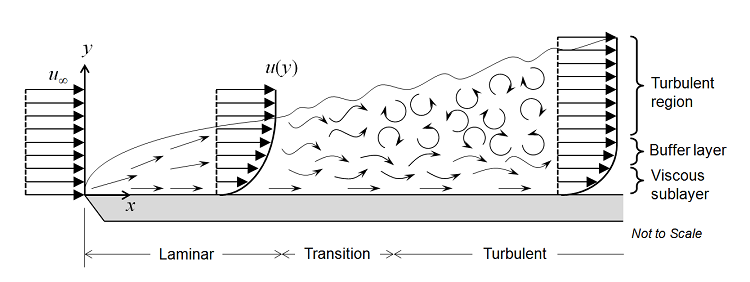
\includegraphics[scale=0.6]{Figures/BL_laminar_turbulent.png}
    \caption{The Development of a Boundary Layer Along Flat Plate \cite{Frei2017WhichApplication}.}
    \label{fig:3}
\end{figure}

 
\noindent From Figure~\ref{fig:3}, it can be seen that there are two main types of boundary layer flow: laminar and turbulent. Laminar is seen close to the leading edge, where the fluid travels smoothly, showing a low velocity gradient and low friction near the wall. When the boundary layer transitions to turbulent, the velocity gradient increases and the friction between the layers becomes significant \cite{Scibor-Rylski1984RoadAerodynamics}. Turbulent flows can be characterised as having irregular and random fluid movement, and showing the presence of eddies. Understanding the boundary layer is essential due to its ability to produce drag due to skin friction. When the local velocity increases, the velocity gradients $(\frac{\partial V}{\partial y})_{y=0} $ and shear stresses near the wall ($\tau_w $) also go up, increasing the overall drag.

\noindent It has to be noted that turbulent flow and separated flow are related but different flow phenomena. Flow separation occurs when the boundary layer detaches from a surface, typically when the surface geometry is curving away. When the air stream decelerates, the pressure gradient acts against the flow direction, creating an adverse pressure gradient, which goes on to cause a thickening of the boundary layer \cite{Scibor-Rylski1984RoadAerodynamics}. At some point the shear stress (friction) and adverse pressure gradient cause the fluid to recirculate. At this stage, the boundary layer separates and creates a region of reversed flow. This condition is illustrated in Figure~\ref{fig:flow separation}.

\begin{figure}[!ht]
    \centering
    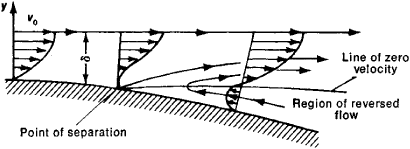
\includegraphics[scale= 0.7]{Figures/flow_separation.png}
    \caption{Illustration of Separated Flow Formation Along Curved Body \cite{Anonymous1979SeparationDictionary}.}
    \label{fig:flow separation}
\end{figure}

\subsubsection{Bernoulli Equation \& Venturi Effect}
Bernoulli's equation is another critical piece of mathematical analysis that quantifies the relationship between flow speed and pressure. This is fundamental to the aerodynamics of undertrays. For inviscid, incompressible flows, the equation can be expressed as:
\begin{equation}
   \underbrace{p}_\textrm{Static Pressure} + \underbrace{\frac{1}{2} \rho V^{2}}_{\substack{\text{Kinetic Energy} \\ \text{per Unit Volume}}} + \underbrace{\rho g h}_{\substack{\text{Potential Energy} \\ \text{per Unit Volume}}} = \text{constant}
    \label{eq:bernoulli}
\end{equation}

\noindent Equation~\ref{eq:bernoulli} clearly illustrates the relationship between speed and pressure when the flow's density can be assumed constant. The equation states that pressure is inversely proportional to the square of the airspeed --- therefore, an increase in velocity has to be accompanied by a reduction in pressure and vice versa. This strongly connected to the generation of downforce in an undertray: flow acceleration underneath a car will reduce the pressure, and hence produce downforce.  Bernoulli's equation only applies to inviscid flow (no consideration of viscosity) which is not a reasonable assumption of undertrays, however, the fundamental understanding of the behaviour of a car's underbody can be gained.

\noindent The underbody of a racing car can be thought of as a Venturi tunnel, where the airflow goes underneath the car into a converging area, and is then expanded at the rear, as illustrated in Figure~\ref{fig:venturi_tunnel_car}. This shape aims to promote the Venturi effect in the proximity of the ground, which increases the downforce and reduces drag \cite{Katz2005AerodynamicsCars}. The continuity formula $\rho AV = \text{constant}$ states that the reduction in underbody cross-sectional area increases the velocity, and hence decreases the pressure (from Equation~\ref{eq:bernoulli}).

\begin{figure}[!ht]
    \centering
    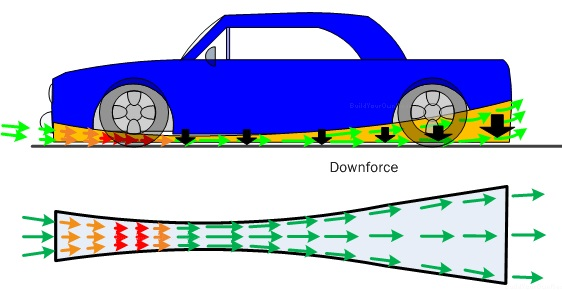
\includegraphics[scale=0.8]{Figures/venturi_tunnel.jpg}
    \caption{Venturi Tunnel Modelling of an Automotive Underbody \cite{Anonymous2020RaceDesign}.}
    \label{fig:venturi_tunnel_car}
\end{figure}

\noindent It is worth noting that this simplification only applies in an ideal situation in which the mass of air is fully conserved throughout the undertray. In real-life conditions, there will be some leakages of air from the sides of the undertray, which will create corner vortices that significantly affect overall car performance. Theoretically, best downforce performance is achieved by maximising the cross-sectional area reduction of the inlet and area expansion of the rear, but this is not possible due to viscosity. An aggressive reduction in area near the inlet will accelerate the flow and give a proportional drag increase, whilst a high diffuser area (outlet angle) will create flow separation --- which reduces the downforce and creates a significant wake at the rear of the car, and hence higher drag. To achieve an optimised underbody design, a range of geometrical variables must be widely and deeply analysed to identify their effects on the aerodynamic forces.

\subsubsection{Aerodynamic Forces}
The optimisation of the forces generated by the aerodynamic flow around the car is the main goal of this project. The flow pattern around a body produces a pressure distribution over the surface \cite{Scibor-Rylski1984RoadAerodynamics}, which means that integrating the pressure over the body surface will give the total inviscid forces produced around the body by the flow. The general force equation of a body can be expressed as:
\begin{equation}
    F = qSC_f
\end{equation}
where $C_f$ is a dimensionless coefficient dependent on the body's shape \cite{Scibor-Rylski1984RoadAerodynamics} and $S$ is the area on which the force acts. In an analysis of drag, the surface is usually taken as the frontal area of a body (illustrated on Figure~\ref{fig:Force direction and frontal area} right). On the other hand, the lift analysis generally uses the area of the lift generator (e.g. undertray, inverted wing, or car wetted-surface).

\begin{figure}[!h]
\begin{center}
%    
  \begin{subfigure}[b]{0.4\textwidth}
    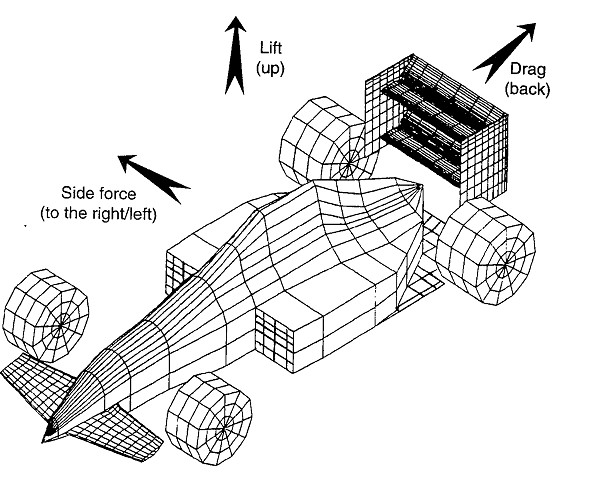
\includegraphics[scale=0.4]{Figures/race_car_forces.jpg}
  \end{subfigure}
  %
  \begin{subfigure}[b]{0.4\textwidth}
    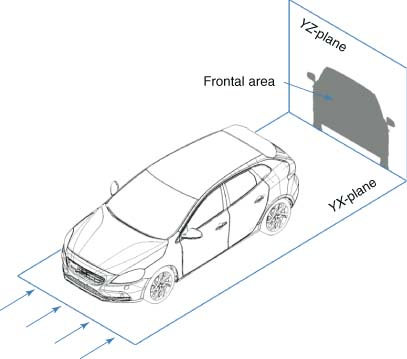
\includegraphics[scale=0.8]{Figures/frontal_area.jpg}
  \end{subfigure}
%  
  \caption{Force Direction Acting On a Race-Car (left) and Representation of Frontal Area of an Automotive Body (right)\cite{Sebben2014FundamentalsDesign}.}
    \label{fig:Force direction and frontal area}
\end{center}
\end{figure}
\noindent There are three main aerodynamic forces acting on a car body: lift, drag, and side force. Figure~\ref{fig:Force direction and frontal area} illustrates the direction of forces acting on a car. Due to the nature of the undertray, having a relatively small effect on side force, this paper will only focus on the generation and optimisation of lift and drag.

\paragraph{Lift (downforce)}
Lift is an applied force due to the pressure difference on a body, which acts vertically and perpendicular to the drag force \cite{Scibor-Rylski1984RoadAerodynamics}. Lift can be mathematically expressed as:
\begin{equation}
    L = \frac{1}{2}\rho U^2 S C_L
\end{equation}
It is important in the motor-sport industry that a racing car produces as much downforce (negative lift) for as little drag possible. In the aviation field, the aerofoil generates positive force to lift the aircraft from the ground, but lift on a race car is used to increase the tyre grip by using an inverse aerofoil concept which produces a downwards force. This consideration is due to the significant improvement in road handling coming from increased tyre grip --- enabling higher cornering speed, acceleration, and more aggressive braking \cite{Barnard1997RoadIntroduction}.


\paragraph{Drag}
Drag is a force that works against the direction of motion of a body, which manifests in friction or pressure distribution \cite{Obidi2014TheoryVehicles}. The drag force is always directed to oppose the car's motion. Drag force can be mathematically expressed as:
\begin{equation}
    D = \frac{1}{2}\rho U^2 S C_D
\end{equation}
If the viscosity of air can be assumed as constant in the analysis, then the only variable that could be modified to reduce the drag are the body's size and geometry. It has to be noted here that racing car drag is usually divided into five different types \cite{Kelly1964AerodynamicsEngineers}: form drag, lift induced drag, surface drag, interference drag, and internal flow drag.

\subsection{Aerodynamic Undertray}
An undertray is an aerodynamic device that is attached to the underside of a racing car to take advantage of accelerating the flow under the car to decrease the pressure and increase the downforce. The undertray has become an important component in the motor-sport industry, as it is used to produce around 45\% of car's downforce \cite{Katz1995RaceSpeed}. A typical undertray consist of a nozzle (inlet), floor section (throat), and diffuser (outlet). Figure~\ref{fig:underbody} shows an example of simple undertrays fitted to  Formula car.

\begin{figure}[!ht]
\begin{center}
%    
  \begin{subfigure}[b]{0.4\textwidth}
    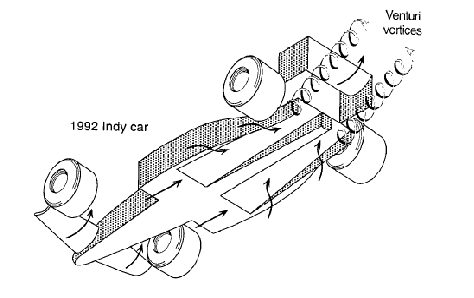
\includegraphics[height=4.5cm]{Figures/underbody.PNG}
  \end{subfigure}
  %
  \begin{subfigure}[b]{0.4\textwidth}
    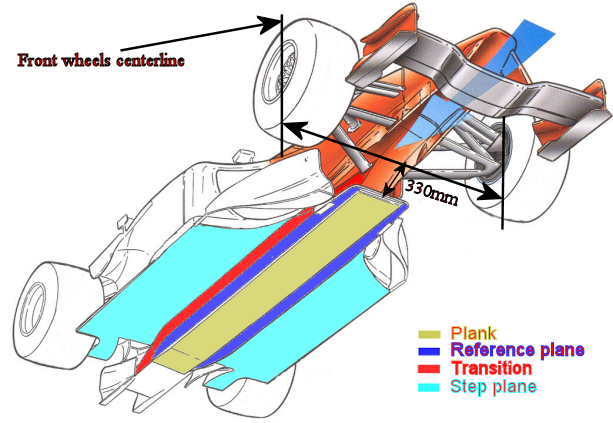
\includegraphics[height=4.5cm]{Figures/undertray_f1.png}
  \end{subfigure}
%  
  \caption{Typical Undertray of a Formula Race-Car \cite{Katz1995RaceSpeed}\cite{AnonymousUndertrayUnderbody}.}
    \label{fig:underbody}
\end{center}
\end{figure}

\noindent As stated before, the Venturi tunnel concept is used by undertrays to generate downforce. The convergent section of the Venturi tunnel produces an increase in velocity, which reduce the pressure on the floor section. This pressure reduction can be significant, and creates a suction-like phenomena which pulls the car down and creates higher traction. On the rear side of the undertray is the divergent section (diffuser), where kinetic energy is converted into a pressure rise. 

\noindent Up until QFR 2021, an undertray has been the only passive aerodynamics device that has actually been produced and attached to the car. The development of these undertrays has been explored in earlier projects in 2017 \cite{McKeown2018DesignCar}, and 2019 \cite{McClune2018DesignCar}. These projects included a number of 2D simulations that tested various geometric variables of the undertray, such as diffuser and inlet angle, and some for the 3D undertray. The case analyses by McKeown \cite{McKeown2018DesignCar}, and McClune \cite{McClune2018DesignCar} were, however, flawed due to the non-existence of the bluff-body. The generation of force on the undertray is affected by the flow passing over the top of the undertray, which makes these analyses unrealistic approximation to the real-life situation \cite{Corr2017MechanicalAuthor}. Therefore, this project will explore the underbody's flow behaviour more accurately, by including a bluff-body with both the 2D and 3D analyses.   

\subsubsection{Undertray Devices}
Typically, race competition rules strictly regulate the geometrical design of undertrays. Formula Student rules are more flexible, and using some kind of aerodynamic devices in the cars can slightly improve the performance. Examples of these kinds of devices are diffuser fences and Gurney flaps.

\noindent Fences or strakes on a diffuser act as a force generator. As discussed previously, the corner vortices at the rear diffuser generate downforce, and the strakes help the diffuser generate more vortices, increasing the downforce. Figure~\ref{fig:gurney} (left) shows an example of a basic strake on a diffuser. A Gurney flap is a small flap or L-shaped structure attached at the end of the diffuser, as shown in Figure~\ref{fig:gurney} (right). Generally, the Gurney flap is used to improve downforce without a significant corresponding rise in drag \cite{Willemsen2012CFD-basedDiffuser} by making the boundary layer stay attached and delaying flow separation to the end of the diffuser by reducing the pressure on the underside of the diffuser, and increasing the pressure on the top of the diffuser. 

\noindent The undertray is one of the most important devices in the high-speed racing industry. The competitive environment between teams in the race-car industry means that proprietary information such as undertray designs are treated as confidential and exclusive to the team; hence, this creates an informational gap in the field. This phenomenon is shown by the lack of open-research papers available to the public.

\begin{figure}[!ht]
\begin{center}
%    
  \begin{subfigure}[b]{0.4\textwidth}
    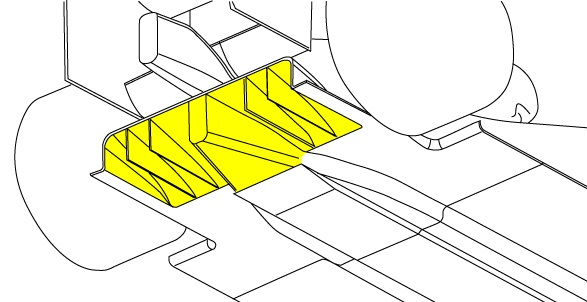
\includegraphics[scale=0.6]{Figures/diffuser_fences.jpg}
  \end{subfigure}
  %
  \begin{subfigure}[b]{0.4\textwidth}
    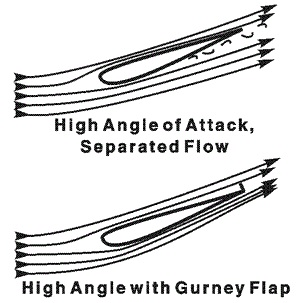
\includegraphics[scale=0.8]{Figures/Gurney.jpg}
  \end{subfigure}
%  
  \caption{Fences or Strake or Vortex Generator on a Diffuser (left) and Example of a Gurney Flap Application on a Wing (right) \cite{Anonymous2020GurneyFlap}.}
    \label{fig:gurney}
\end{center}
\end{figure}